% !TEX root = document.tex

\chapter{\label{chap:introduction}Introduction}
Most audio streaming services are run by single companies, which take large cuts of the subscription money from its users. As a result, the artists receive a low compensation. 

\begin{figure}
	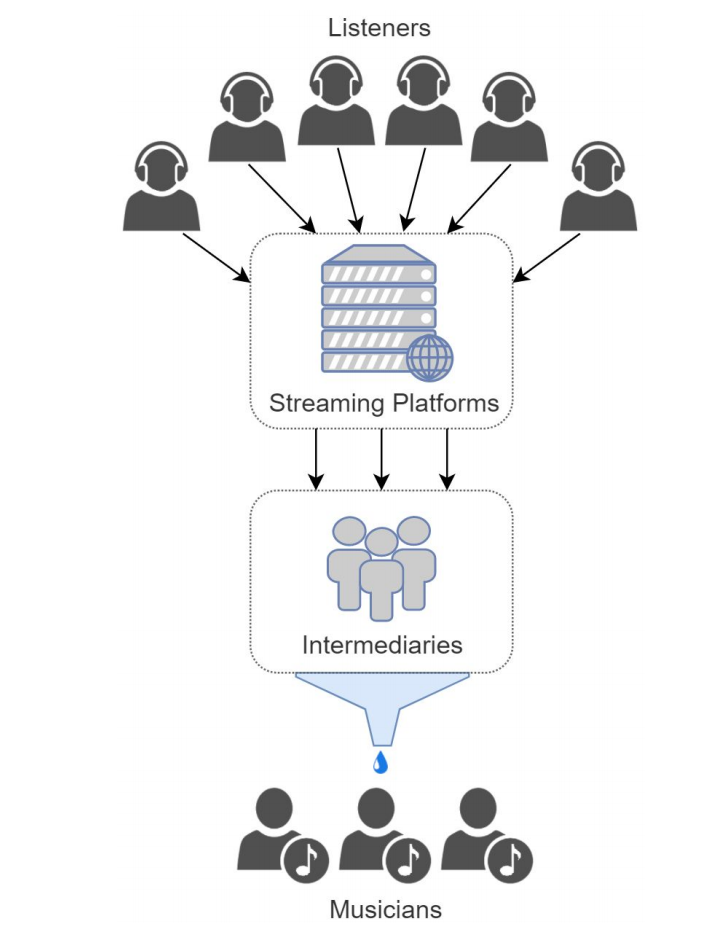
\includegraphics[width=0.4\textwidth]{./img/problem-image.png}
	\caption{Artist compensation inconsistency}
\end{figure}

This thesis proposes a solution in the form of a decentralized system which uses a decentralized autonomous organization \todo{cite}(DAO) to operate. Listeners, artists and robots form this DAO. In this system, its users (artists and listeners) share audio content without any middleman. Additionally, users can give donations to artists while the system does not take a cut of these donations. 

\todo{XYZ} Section X describes the design of the system, section Y its implementation and Z its testing results.